\chapter{连通度}
  \begin{Def}
    图$G$的{\bfseries 顶点连通度}是指为了产生一个不连通图或平凡图所需要从$G$中去掉的最少顶点数目, 记为$\kappa (G)$。
  \end{Def}
  \begin{Def}
    图$G$的{\bfseries 边连通度}是指为了产生一个不连通图或平凡图所需要从$G$中去掉的最少边的数目, 记为$\lambda (G)$。
  \end{Def}
  \begin{Def}
    设$G$是一个图,如果$\kappa (G) \geq n$,则称$G$是{\bfseries $n$-顶点连通}的,简称$n$-连
    通;如果$\lambda (G) \geq n$,则称$G$是{\bfseries $n$-边连通}的。
  \end{Def}

\begin{Ex}
  构造一个图$G$,使得$\kappa(G)=3,\lambda(G)=4,\delta(G)=5$。
\end{Ex}
\begin{proof}[解]
\mbox{} \par \noindent

 \begin{center} 
  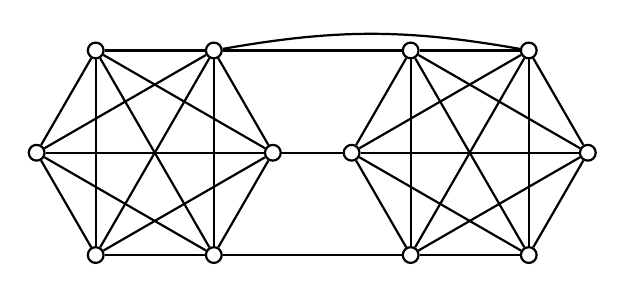
\begin{tikzpicture}[auto,
    specification/.style ={circle, draw, thick, inner sep = 0pt, minimum size=2mm}]
   \node[specification] (A)  at (0:1.5cm)  {};
   \node[specification] (B)  at (60:1.5cm)  {};
   \node[specification] (C)  at (120:1.5cm)  {};
   \node[specification] (D) at (180:1.5cm)  {};
   \node[specification] (E)  at (240:1.5cm)  {};
   \node[specification] (F)  at (300:1.5cm)  {};

   \node[specification] (G)  at ([xshift=4cm]0:1.5cm)  {};
   \node[specification] (H)  at ([xshift=4cm]60:1.5cm)  {};
   \node[specification] (I)  at ([xshift=4cm]120:1.5cm)  {};
   \node[specification] (J) at ([xshift=4cm]180:1.5cm)  {};
   \node[specification] (K)  at ([xshift=4cm]240:1.5cm)  {};
   \node[specification] (L)  at ([xshift=4cm]300:1.5cm)  {};

   
   \draw[thick] (A) to  (B);
   \draw[thick] (A) to  (C); 
   \draw[thick] (A) to  (D);
   \draw[thick] (A) to  (E);
  
   \draw[thick] (B) to  (C);
   \draw[thick] (B) to  (D);
   \draw[thick] (B) to  (E);
   \draw[thick] (B) to  (F);
  
   \draw[thick] (C) to  (D);
   \draw[thick] (C) to  (E);
   \draw[thick] (C) to  (F);
   


   \draw[thick] (D) to  (E);
   \draw[thick] (D) to  (F);
   \draw[thick] (E) to  (F);
   \draw[thick] (F) to  (A);

   \draw[thick] (G) to  (H);
   \draw[thick] (G) to  (I);
   \draw[thick] (G) to  (J);
   \draw[thick] (G) to  (K);


   
   \draw[thick] (H) to  (I);
   \draw[thick] (H) to  (J);
   \draw[thick] (H) to  (K);
   \draw[thick] (H) to  (L);
   
   \draw[thick] (I) to  (J);
   \draw[thick] (I) to  (K);
   \draw[thick] (I) to  (L);
   


   \draw[thick] (J) to  (K);
   \draw[thick] (J) to  (L);
   
   \draw[thick] (K) to  (L);

   \draw[thick] (L) to  (G);

   \draw[thick] (A) to  (J);
   \draw[thick] (F) to  (K);
   \draw[thick] (B) to  (I);
   \draw[thick] (B) to [bend left = 10] (H);
 \end{tikzpicture}
\end{center}
  
\end{proof}

%%% Local Variables:
%%% mode: latex
%%% TeX-master: "book"
%%% End: